\begin{frame}
\frametitle{"Projet long" background}
\begin{block}{THC 2018 Challenge}
\begin{itemize}
\item Prepare tutorial challenge
\item Work based on \textit{GSMem: Data Exfiltration from Air-Gapped 
Computers over GSM Frequencies} (24th USENIX Security Symposium)
\item "Challenge" : data exfiltration form an air-gapped computer
\item "Tutorial" : guide the challenger step-by-step
\item Idea : follow how we succeed to reproduce a part of the paper
\end{itemize}
\end{block}
\end{frame}

\begin{frame}
\frametitle{Electromagnetic emanations}
\begin{block}{Emanations}
\begin{itemize}
\item Each electronic device has emanations
\item Could be electronical, acoustical, mecanical or electromagnetical
\item We focused on electromagnetic emanations
\end{itemize}
\end{block}

\begin{block}{TEMPEST}
\begin{itemize}
\item Name given by NSA for standards protecting against electromagnetic emanations
\item Context : EMSEC, surbpart of COMSEC
\end{itemize}
\end{block}
\end{frame}


\begin{frame}
\frametitle{Air-gapped networks}
\centering 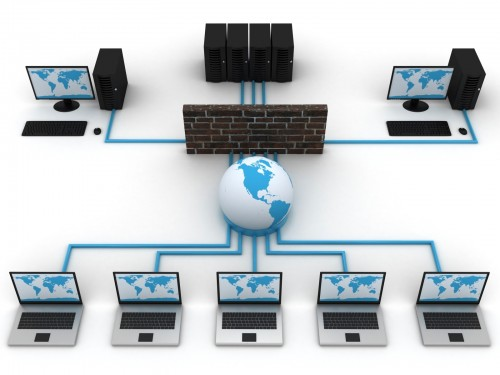
\includegraphics[scale=.5]{images/network.jpg}
\end{frame}

\begin{frame}
\frametitle{Air-gapped networks}
\centering 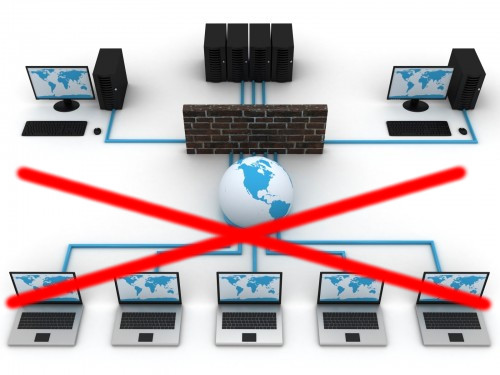
\includegraphics[scale=.5]{images/network2.jpg}
\end{frame}


\begin{frame}
\frametitle{Data exfiltration}
\begin{block}{Devices}
\begin{itemize}
\item 1 air-gapped computer (attacked computer)
\item 1 standard computer (attacker's computer)
\end{itemize}
\end{block}

\begin{block}{Tools}
\begin{itemize}
\item Spectrum analyzer
\item Software-defined radio : USRP/RTL-SDR
\item Antennas
\item Softwares : URH/GNURadio
\end{itemize}
\end{block}

\begin{block}{Goal}
Transfer a password from the air-gapped computer to the attacker's computer creating a covert channel.
\end{block}

%\begin{center}
%
\includegraphics[scale=.37]{images/com.pdf}
%\end{center}
\end{frame}